\chapter{Exercício 5}
\label{cha:exercise_5}

\section{Configuração de um servidor HTTPS e autenticação de cliente}

O objetivo deste exercício consiste em configurar um servidor HTTPS recorrendo ao código disponibilizado no repositório da disciplina, utilizando o certificado e chave privada correspondentes ao domínio \texttt{www.secure-server.edu}, emitidos pela CA1-int do primeiro trabalho. O servidor é configurado em dois cenários distintos:  
1) sem autenticação de cliente  
2) com autenticação de cliente usando o certificado \texttt{Alice\_2}.

A implementação do servidor, realizada em Node.js, permite ajustar diretamente os parâmetros do handshake TLS através do objeto \texttt{options}. A configuração inclui a chave privada do servidor, o respetivo certificado e a cadeia da autoridade certificadora responsável pela sua emissão.

\subsection{Configuração sem autenticação de cliente}

No primeiro cenário, o servidor HTTPS é configurado para não exigir qualquer certificado ao cliente. Neste modo, os parâmetros relevantes do handshake são:

\begin{itemize}
    \item \texttt{requestCert = false}: o servidor não solicita certificado ao cliente.
    \item \texttt{rejectUnauthorized = false}: mesmo que algum certificado fosse enviado, não seria verificado.
\end{itemize}

Nesta configuração, a comunicação estabelece-se garantindo confidencialidade e integridade, mas sem autenticação do cliente.

A ligação foi testada com um browser, confirmando que o acesso ao servidor é realizado sem qualquer pedido de certificado. O ecrã correspondente encontra-se aqui: 
\begin{figure}[h]
    \centering
    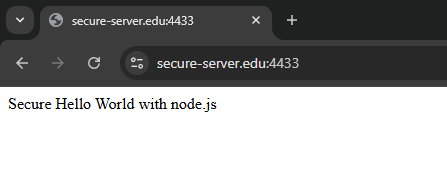
\includegraphics[width=0.75\textwidth]{images/noauth.png}
    \caption{Ligação bem-sucedida ao servidor HTTPS sem pedido de certificado do cliente}
    \label{fig:noauth}
\end{figure}

Para esta configuração, adicionamos o certifcado CA1 à lista de cerificados de autoridades
de certificação de raiz fidedigna do sistema operativo.

\subsection{Configuração com autenticação de cliente}

No segundo cenário, o servidor é configurado para exigir autenticação mútua TLS (mTLS). Os parâmetros alterados foram:

\begin{itemize}
    \item \texttt{requestCert = true}: o servidor solicita um certificado ao cliente.
    \item \texttt{rejectUnauthorized = true}: o servidor valida o certificado usando a CA fornecida.
    \item \texttt{ca = fs.readFileSync('ca2.pem')}: é usada a CA que emitou o certificado \texttt{Alice\_2}.
\end{itemize}

Com esta configuração, o browser solicita ao utilizador a seleção de um certificado válido, sendo usado o certificado \texttt{Alice\_2}. A ligação só é concluída se o certificado pertencer à cadeia confiada pelo servidor.

A captura de ecrã demonstrando a ligação com autenticação de cliente encontra-se aqui: 


% Imagem do browser pedindo certificado
\begin{figure}[h]
    \centering
    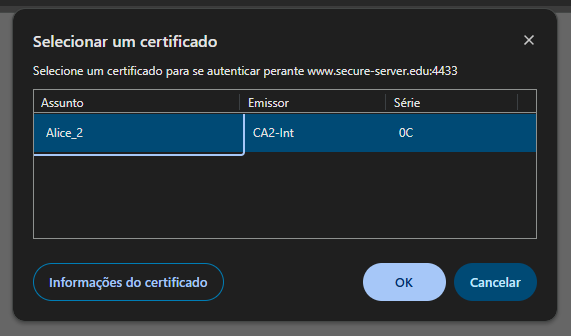
\includegraphics[width=0.75\textwidth]{images/pedidoCertificado.png}
    \caption{Prompt do browser solicitando o certificado do cliente (\texttt{Alice\_2})}
    \label{fig:pedidoCertificado}
\end{figure}

Após a seleção correta do certificado, a ligação é estabelecida com sucesso.

% Imagem do browser após autenticação
\begin{figure}[h]
    \centering
    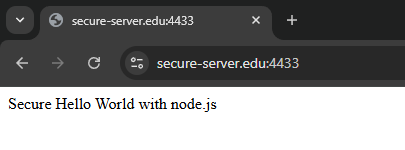
\includegraphics[width=0.75\textwidth]{images/withAuth.png}
    \caption{Ligação bem-sucedida ao servidor HTTPS com autenticação do cliente}
    \label{fig:withAuth}
\end{figure}

Para esta configuração, adicionamos a chave privada \texttt{Alice\_2} à lista de cerificados pessoais do utilizador
autenticado no sistema operativo. E, ainda, adicionamos o cerificado CA2-Int à lista de cerificados de autoridades
de certificação intermédias do sistema operativo.

\subsection{(i) Algoritmos de segurança usados no Record Protocol}

Ao ligar o browser ao servidor HTTPS, a análise do Security Overview revela os seguintes parâmetros de segurança:

\begin{itemize}
    \item \textbf{Protocolo}: TLS 1.3
    \item \textbf{Troca de chaves}: X25519 (ECDHE)
    \item \textbf{Cifra de sessão}: AES-256-GCM
\end{itemize}

\paragraph{Confidencialidade das mensagens:}
A confidencialidade é assegurada pelo algoritmo AES-256 em modo GCM, um esquema AEAD (Authenticated Encryption with Associated Data) que cifra os dados e impede que um atacante obtenha o conteúdo sem possuir as chaves de sessão derivadas durante o handshake.

\paragraph{Autenticidade e integridade:}
O modo GCM fornece tanto integridade como autenticidade através do \textit{authentication tag}, detectando qualquer alteração nos dados transmitidos. Em TLS 1.3 não é necessário HMAC separado, pois toda a proteção de integridade é gerida pelo AEAD.

\paragraph{Estabelecimento de chaves e Perfect Forward Secrecy:}
A troca de chaves é feita via X25519, variante de ECDHE, garantindo Perfect Forward Secrecy (PFS). Mesmo que a chave privada do servidor seja comprometida no futuro, comunicações passadas não podem ser decifradas.

\paragraph{Autenticação dos participantes}
\begin{itemize}
    \item \textbf{Sem autenticação de cliente}: apenas o servidor é autenticado através do seu certificado X.509.
    \item \textbf{Com autenticação de cliente}: o browser apresenta o certificado Alice\_2, que é validado pelo servidor, garantindo autenticação do cliente.
\end{itemize}

\subsection{(ii) Vulnerabilidade da cipher suite TLS\_RSA\_WITH\_AES\_128\_CBC\_SHA256}

Esta suite utiliza RSA clássico para troca de chaves. O problema central consiste no facto de:

\[
\text{premaster secret} \longrightarrow \text{RSA-encryptado diretamente com } PK_{Server}
\]

Se o atacante registar o tráfego TLS e mais tarde obtiver a \textbf{chave privada RSA do servidor}, pode executar:

\[
\text{premaster secret} = D_{SK_{Server}}(\text{ClientKeyExchange})
\]

Depois de recuperar o premaster secret, todo o tráfego TLS pode ser decifrado retroativamente, sendo possível reconstruir as chaves simétricas derivadas na fase de handshake. Este ataque denomina-se \textit{RSA key exchange compromise} e é a principal razão pela qual RSA deixou de ser recomendado para troca de chaves em TLS 1.3, sendo substituído por esquemas ECDHE que garantem confidencialidade perfeita (PFS).

Assim, um atacante com acesso posterior à chave privada do servidor pode decifrar comunicações passadas entre browser e servidor, comprometendo confidencialidade histórica.

\section{Ligação a servidor HTTPS usando JCA}

A alínea 5.2 exige a implementação de um cliente HTTPS em Java utilizando a API JCA (Java Cryptography Architecture), capaz de se ligar ao servidor HTTPS configurado previamente, no modo sem autenticação de cliente.

A aplicação Java carrega uma truststore contendo exclusivamente a CA que emitiu o certificado do servidor. Esta truststore, \texttt{roots.jks}, foi obtida no trabalho anterior e substitui a necessidade de criar um novo ficheiro com \texttt{keytool}. O cliente realiza:

\begin{enumerate}
    \item carregamento explícito da truststore;
    \item criação de um \texttt{TrustManagerFactory};
    \item inicialização de um \texttt{SSLContext} com os gestores de confiança;
    \item estabelecimento de um \texttt{SSLSocket} para o servidor \texttt{localhost:4433};
    \item execução do handshake TLS;
    \item obtenção da sessão TLS negociada.
\end{enumerate}

Depois da ligação, o programa imprime o protocolo TLS e a cipher suite efetivamente negociada.

A execução da aplicação produziu o seguinte resultado:

\begin{verbatim}
Protocolo:    TLSv1.3
Cipher Suite: TLS_AES_256_GCM_SHA384
\end{verbatim}

A suite \texttt{TLS\_AES\_256\_GCM\_SHA384} é característica de TLS 1.3 e utiliza AES no modo GCM, que garante simultaneamente confidencialidade, integridade e autenticidade das mensagens sem necessidade de HMAC separado.
